\chapter{Testing}
\label{chp:testing}
\section{Strategy}
% Justification for different kinds of test
% What my plan was before I did the testing
The approach used for testing each of the components was limited to unit testing. Having previous experience with unit testing in both Java and Python lead to this decision.  The plan for testing the plugin was simple; test each of the detection methods. The plan for testing the server was to test each of the Flask routes to ensure the correct outcome. The post-processor acts as an I/O tool so the plan is to simply test that I/O process. Due to the lack of experience with setting up CI (continuous integration), this was considered but not set up. This would have eased with ensuring breaking changes are accepted. However, both the server and post-processor will be built as Docker containers and will run the tests as they are built. Any failing tests will fail the build.

\section{Plugin}
JUnit was used for testing the plugin. The IntelliJ Plugin SDK provides a testing infrastructure. This allows testing the plugin in a headless environment. What this means is that the IDE is run without the UI to test all aspects of the plugin. Everything is loaded as usual except the UI. The SDK provides classes and methods to \textit{emulate} user actions such as typing, pasting, clicking menu items, and clicking tool bar buttons. Emulating such actions allows testing of detecting editor changes.

Four classes are included in the tests directory. \texttt{BaseClass} provides useful assertion methods. These will check file changes for specific data. \texttt{CipherTest} is a simple test case for the 128-bit AES encryption on the tracked data. Encrypted and unencrypted sample data is used to test the both the encryption and decryption methods. \texttt{CopyPasteDetectionTest.java} is a core source detection test for detecting copy-paste in the editor. This ensures that all copy-paste actions in the editor are tracked properly. \texttt{ExternalDetectionTest} is another core source detection test for detecting external file changes. This test is a unique test because it needs to simulate externally changing a file without using the IDE editor. This works by notifying the \texttt{ProjectDocumentListener} that the project has closed, making the changes (and therefore making "external" changes), notify the \texttt{ProjectDocumentListener} that the project is opened, which will detect the "external" changes correctly.

\section{Server}
Nose was used for testing the back-end server. Nose extends unittest to provide extra functionality. Unittest is built-in to Python 3 and works in a similar manner to JUnit. Mock is a library used to replace parts of the system to change functionality. MockupDB is a library used to mock a MongoDB client.

\texttt{base.py} provides generic \texttt{setUp} and \texttt{tearDown} methods, as well as a method to mock or patch the Aberystwyth LDAP connection. This is useful so that the Aberystwyth LDAP server is no directly contacted but instead is replaced with specific values to return. This removes the need to be connected to the Aberystwyth network when running the unit tests, and any username/password combination may be used for tests. \texttt{test\_data.py} has all necessary testing data for the unit tests.

\texttt{test\_auth.py} contains functions which test the LDAP authentication system. The LDAP connection is patched to provide the necessary user information. The scenarios that are tested are: existing user sign-in, first time user sign-in, invalid user credentials sign-in, checking if user is a staff, and checking if user is a student.

\texttt{test\_dashboard.py} provides functions to test the staff and student dashboard routes. This involves sending various POST and GET requests to sign-in, and view the dashboard. The various database requests are received and the necessary data is sent as a reply to each request. The dashboard request is checked to ensure adequate data in the submissions table.

\section{Post-Processor}
Nose was also used for testing the post-processor module due to it also being developed with Python 3. MockupDB is also used for mocking the MongoDB client if necessary. The \texttt{base.py} class is very similar but does not have the function for patching the LDAP connection as this is not used in the post-processor. \texttt{test\_process.py} will test the processing of a submission to ensure the result is as expected. The input as an encrypted XML sample string and the expected output is a dictionary containing the results. The input is processed and the return value is tested.

\section{Results}
\autoref{fig:tests-plugin}, \autoref{fig:tests-post-processor}, and \autoref{fig:tests-server} show that all of the unit tests for each module pass successfully. \autoref{fig:server-terminal-1} and \autoref{fig:server-terminal-2} shows the output from running Docker Compose to deploy the containers.

\begin{figure}[H]
  \centering
  \fbox{
    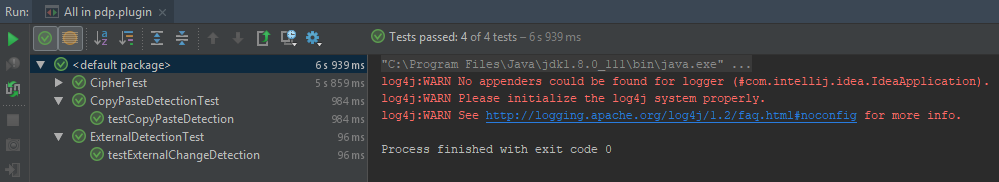
\includegraphics[height=\textheight,
    keepaspectratio=true,
    width=\textwidth,
    ]{figures/00-tests-plugin.png}
  }
  \caption[Plugin tests]{IntelliJ Plugin JUnit tests output}
  \label{fig:tests-plugin}
\end{figure}

\begin{figure}[H]
  \centering
  \fbox{
    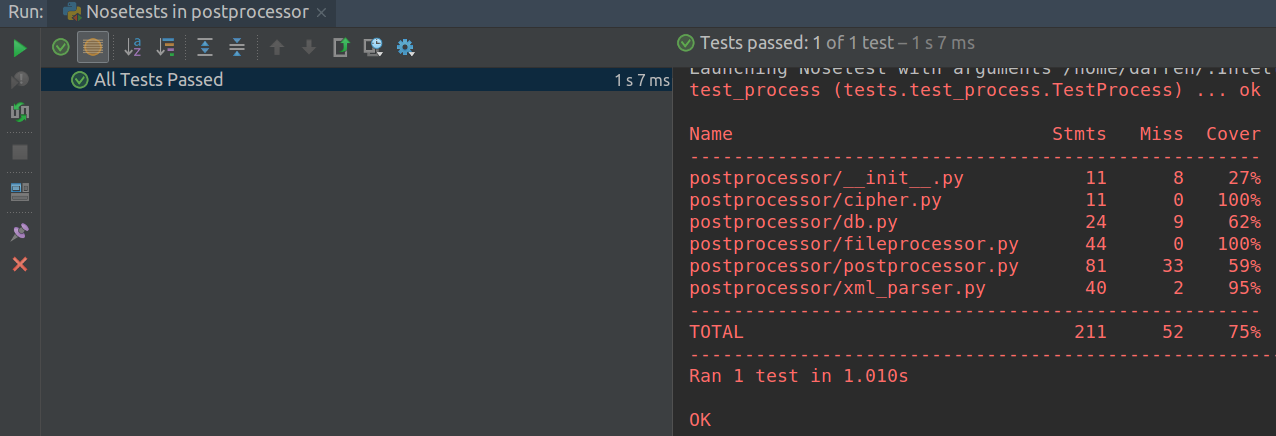
\includegraphics[height=\textheight,
    keepaspectratio=true,
    width=\textwidth,
    ]{figures/01-tests-post-processor.png}
  }
  \caption[Post-processor tests]{Post-processor nose unit tests output}
  \label{fig:tests-post-processor}
\end{figure}

\begin{figure}[H]
  \centering
  \fbox{
    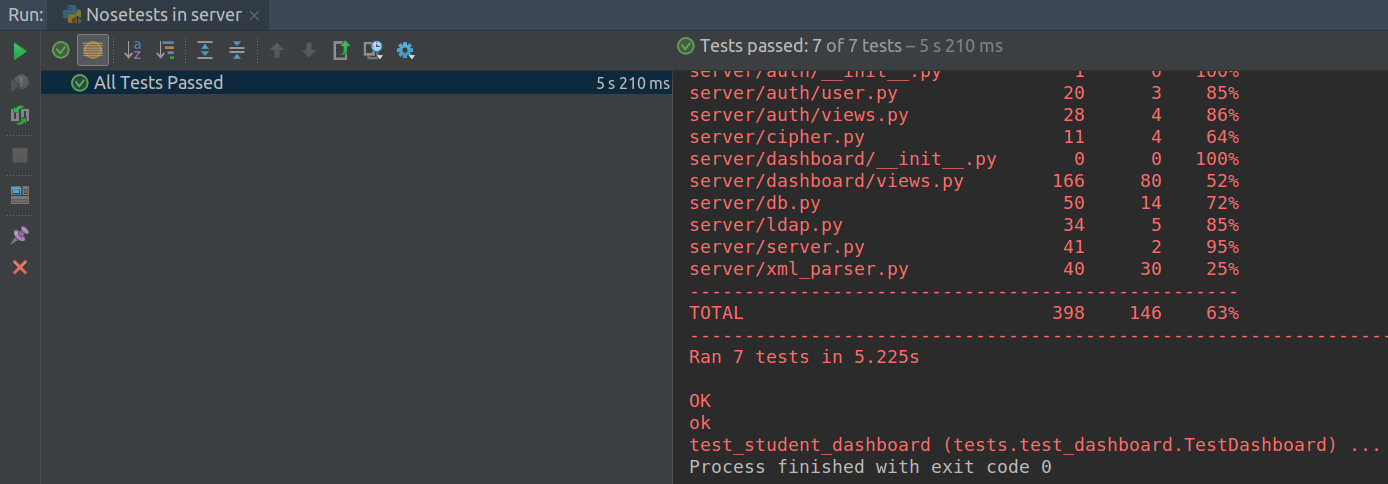
\includegraphics[height=\textheight,
    keepaspectratio=true,
    width=\textwidth,
    ]{figures/02-tests-server.png}
  }
  \caption[Server tests]{Server nose unit tests output}
  \label{fig:tests-server}
\end{figure}

\begin{figure}[H]
  \centering
  \fbox{
    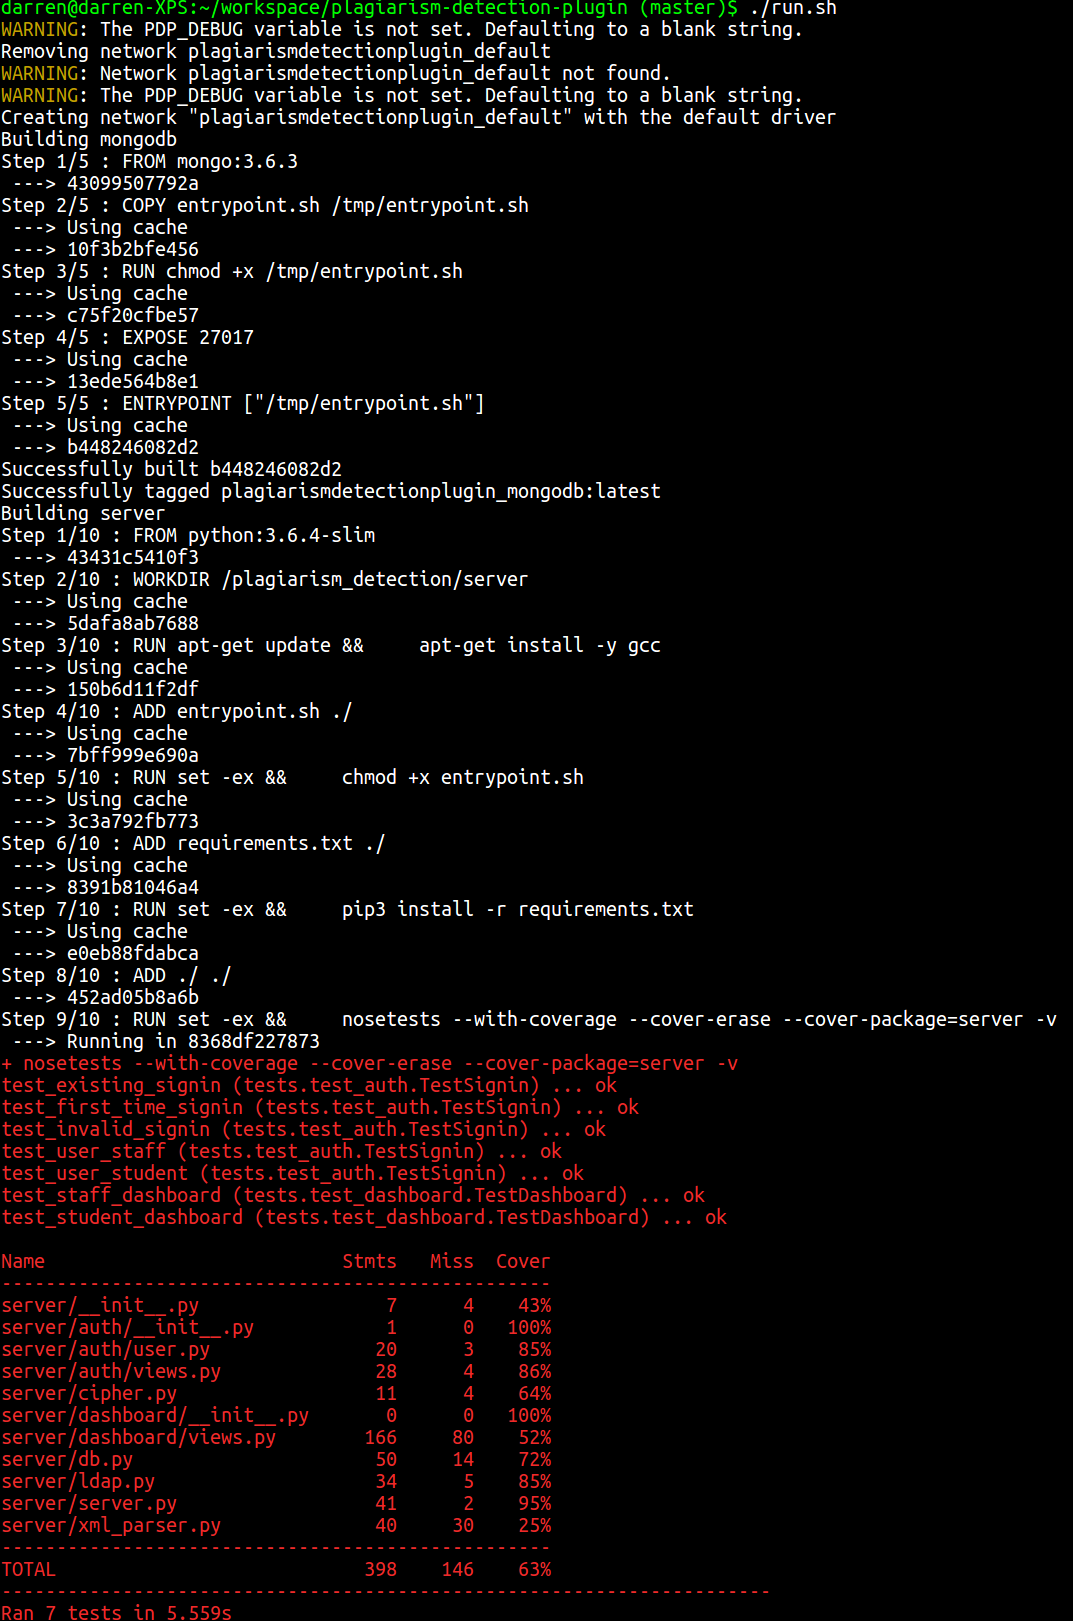
\includegraphics[height=.9\textheight,
    keepaspectratio=true,
    width=.9\textwidth,
    ]{figures/03-server-terminal-1.png}
  }
  \caption[Server Terminal Output 1]{Using Docker Compose to deploy the server}
  \label{fig:server-terminal-1}
\end{figure}

\begin{figure}[H]
  \centering
  \fbox{
    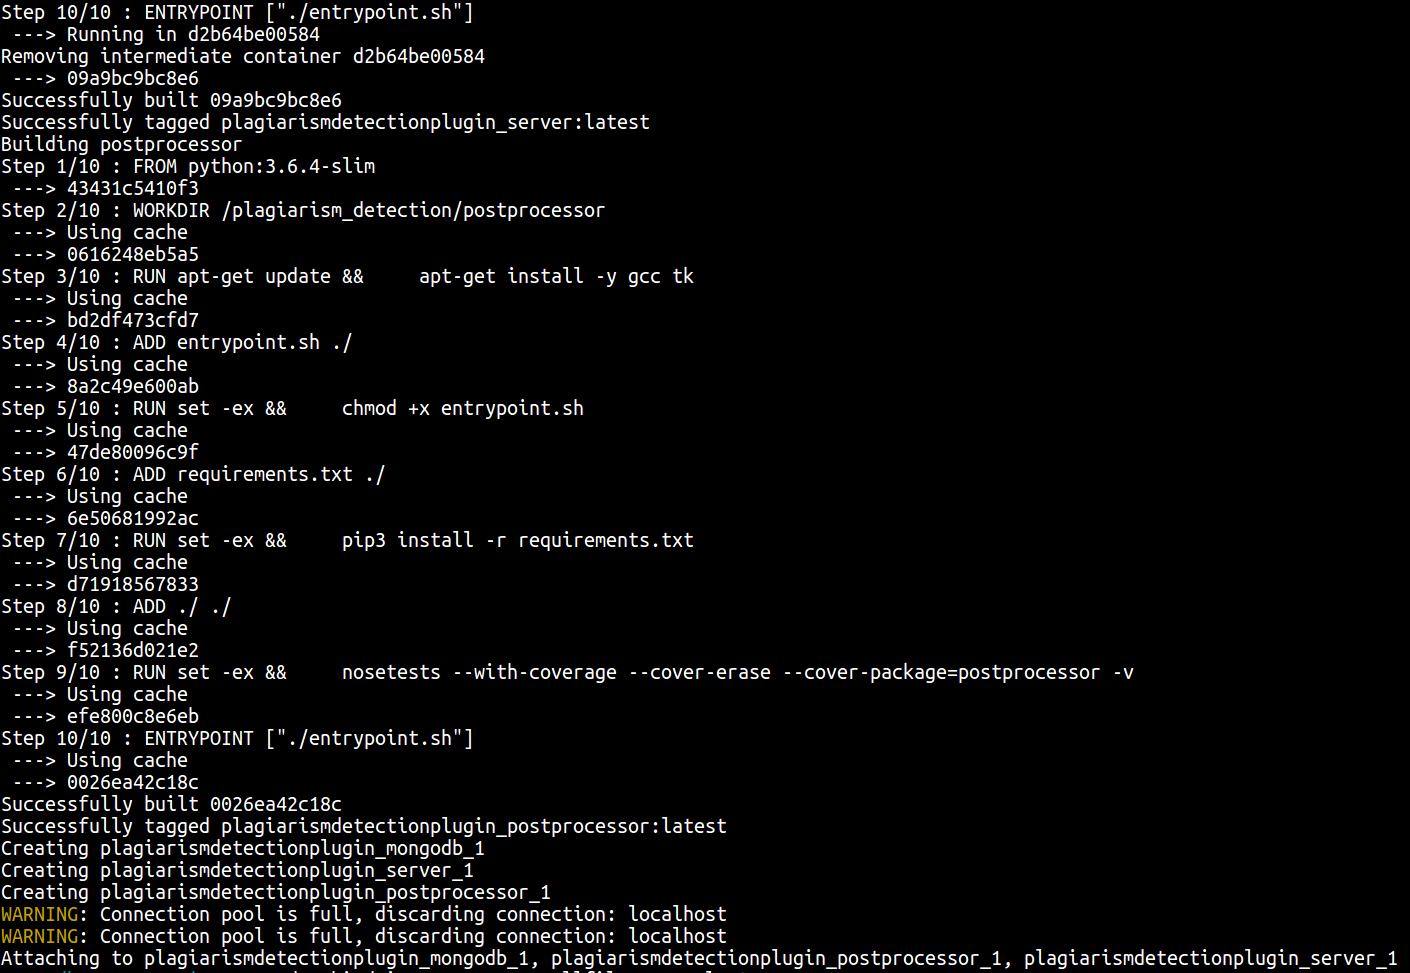
\includegraphics[height=.9\textheight,
    keepaspectratio=true,
    width=.9\textwidth,
    ]{figures/04-server-terminal-2.png}
  }
  \caption[Server Terminal Output 2]{Using Docker Compose to deploy the server}
  \label{fig:server-terminal-2}
\end{figure}


